\documentclass[border=1pt]{standalone}
\usepackage{tikz}


\begin{document}
  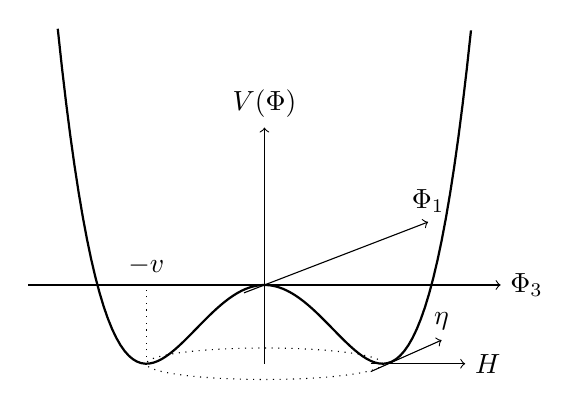
\begin{tikzpicture}[scale=1,xscale=1.5]
    \draw[->] (-2,0) -- (2,0) node[right] {$\Phi_3$};
    \draw[->] (-0.866025*0.2,-0.5*0.2) -- (0.866025*1.6,0.5*1.6) node[above] {$\Phi_1$};
    \draw[->] (0,-1) -- (0,2) node[above] {$V(\Phi)$};
    \draw[dotted] (-1,-1) -- (-1,0) node[above] {$-v$};
    \draw[dotted] (0,-1) ellipse (1 and 0.2);
    \draw[->] (0.9,-1) -- (1.7,-1) node[right] {$H$};
    \draw[->] (0.9,-1.1) -- (1.5,-0.7) node[above] {$\eta$};
    \draw[domain=-1.75:1.75,samples=100,thick,variable=\x] plot ({\x},{-2*\x*\x + \x*\x*\x*\x});
  \end{tikzpicture}
\end{document}